\section{Desarrollo}
\subsection{Teoría}
Para lograr los efectos necesarios, las coordenas de la imagen original deben ser modificadas mediante una transformación lineal seguida de una traslación (lo que comúnmente se conoce como \textit{transformación afín}).

\par La transformación utilizada puede verse en la figura~\ref{fig:transformacion1}. Los valores $a, b, c, d$ son los coeficiententes de transformación, $(x ,y)$ son las coordenadas originales, $x_{0}$ e $y_{0}$ son el offset y $x$', $y$' son las coordenadas resultantes.     

\begin{figure}[h!]
 \caption{Transformación utilizada}
 \centering
   $
   \begin{bmatrix}
x'\\y' 

\end{bmatrix}
=
\begin{bmatrix}
 a & b  & x_{0} \\ 
 a & b  & y_{0} 
\end{bmatrix}
\begin{bmatrix}
x - x_{0}\\ 
y - y_{0}\\
1 
\end{bmatrix}
   $
\end{figure}

En nuestro caso, los coeficientes de transformación deben ser configurados para que la ecuación quede como en la figura~\ref{fig:transformacion2} 

\begin{figure}[h!]
 \caption{Transformación con los coeficientes}
 \centering
 $
 \begin{bmatrix}
x'\\y' 

\end{bmatrix}
=
   \begin{bmatrix}
 \cos \alpha & \sin\alpha  & x_{0} \\ 
 -\sin \alpha & \cos\alpha  & y_{0} 
\end{bmatrix}
\begin{bmatrix}
x - x_{0}\\ 
y - y_{0}\\
1 
\end{bmatrix}
$
   \label{fig:transformacion2}
\end{figure}

\subsection{Detalles de la implementación}
Uno de los primeros temas a solucionar fue cómo calcular los valores de las funciones seno y coseno. La solución consistió en guardar en dos tablas $360$ valores correspondientes a parámetros angulares para dichas funciones (de 0 a 359 grados). Cada resultado se guardó en 16 bits en forma signo más magnitud, con 7 bits para la parte entera y 8 para la decimal. La imagen a cargar es de 64 por 64 pixeles, y cada pixel tiene tres bits para el canal rojo, tres bits para el verde y dos para el azul. Esto resulta en un bitmap que tiene 4096 valores de 8 bits. En la figura~\ref{fig:chess} se puede observar el bitmap utilizado 

\begin{figure}[h!]
 \caption{bitmap utilizado}
 \centering
   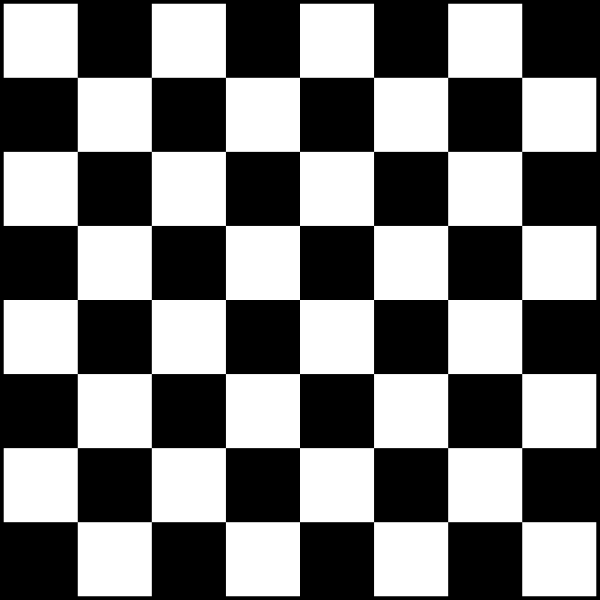
\includegraphics[width=0.5\textwidth]{chessw.png}
   \label{fig:chess}
\end{figure}   